\documentclass[12pt]{ociamthesis}  % default square logo 
%\documentclass[12pt,beltcrest]{ociamthesis} % use old belt crest logo
%\documentclass[12pt,shieldcrest]{ociamthesis} % use older shield crest logo

%load any additional packages
\usepackage{amssymb}
\usepackage{graphicx}


%input macros (i.e. write your own macros file called mymacros.tex 
%and uncomment the next line)
%\include{mymacros}

\title{Hierarchical \\[1ex]Leader Election Algorithm \\[1ex]     %your thesis title,
        With Remoteness Constraint}   %note \\[1ex] is a line break in the title

\author{Mohamed Tbarka}             %your name
\college{ENSIAS}  %your college

%\renewcommand{\submittedtext}{change the default text here if needed}
\degree{Engineering Diplomat}     %the degree
\degreedate{2019}         %the degree date

%end the preamble and start the document
\begin{document}

%this baselineskip gives sufficient line spacing for an examiner to easily
%markup the thesis with comments
\baselineskip=18pt plus1pt

%set the number of sectioning levels that get number and appear in the contents
\setcounter{secnumdepth}{3}
\setcounter{tocdepth}{3}


\maketitle                  % create a title page from the preamble info
\begin{dedication}
This thesis is dedicated to\\
my grand father\\
for inspiring me.\\
\end{dedication}        % include a dedication.tex file
\begin{acknowledgements}
I would like to thank the all library media specialists for their participation in the survey who supported my work in this way and helped me get results of better quality. I am also grateful to the members of my committee for their patience and support in overcoming numerous obstacles I have been facing through my research

I would like to thank my fellow doctoral students for their feedback, cooperation and of course friendship. In addition I would like to express my gratitude to the staff of INFRES-Telecom ParisTech for  the last minute favors.

Nevertheless, I am also grateful to the Mr Petr Kuznetsov for sharing his dissertation woes, and a glimmer of hope for post-dissertation normalcy. I am also thankful to Mrs Sanaa ElFkihi for his efficient supervising.

I would like to thank my friends for accepting nothing less than excellence from me. Last but not the least, I would like to thank my family: my parents and to my brothers and sister for supporting me spiritually throughout writing this thesis and my my life in general.
\end{acknowledgements}   % include an acknowledgements.tex file
\begin{abstract}
A hierarchical algorithm for electing a leaders' hierarchy in an asynchronous network with dynamically changing communication topology is presented including a remoteness's constraint towards each leader. The algorithm ensures that, no matter what pattern of topology changes occur, if topology changes cease, then eventually every connected component contains a unique leaders' hierarchy. The algorithm combines ideas from the Temporally Ordered Routing Algorithm (TORA) for mobile ad hoc networks with a wave algorithm, all within the framework of a height-based mechanism for reversing the logical direction of communication links. Moreover, an improvement from the algorithm in is the introduction of logical clocks as the nodes’ measure of time, instead of requiring them to have access to a common global time. This new feature makes the algorithm much more flexible and applicable to real situations, while still providing a correctness proof. It is also proved that in certain well behaved situations, a new leader is not elected unnecessarily.
\end{abstract}


\newpage

\renewcommand{\abstractname}{Résumé}

\begin{abstract}
Un algorithme hiérarchique pour l'élection d'une hiérarchie de "leaders" dans un réseau asynchrone avec une topologie de communication en évolution dynamique est présenté, incluant une contrainte d'éloignement vis-à-vis de chaque leader. L'algorithme garantit que, quel que soit le modèle de modification de la topologie utilisé, si cette modification cesse, tous les composants connectés contiennent m hiérarchie de leaders unique. L'algorithme combine des idées de l'algorithme TORA (Temporally Ordered Algorithm) pour les réseaux ad hoc mobiles avec un algorithme d'onde, le tout dans le cadre d'un mécanisme basé sur la hauteur destiné à inverser le sens logique des liaisons de communication. De plus, une amélioration de l’algorithme est l’introduction d’horloges logiques comme mesure du temps des noeuds, au lieu de leur demander d’avoir accès à une heure globale commune. Cette nouvelle fonctionnalité rend l'algorithme beaucoup plus flexible et applicable à des situations réelles, tout en fournissant une preuve de correction. Il est également prouvé que dans certaines situations bien conduites, un nouveau "leader" n’est pas élu inutilement.

\end{abstract}


          % include the abstract

\begin{romanpages}          % start roman page numbering
\tableofcontents            % generate and include a table of contents
\listoffigures              % generate and include a list of figures
\end{romanpages}            % end roman page numbering

%now include the files of latex for each of the chapters etc
\chapter{Introduction}

Leader election is an important primitive for distributed computing, useful as a subroutine for any application that requires the selection of a unique processor among multiple candidate processors. Applications that need a leader range from the primary-backup approach to replication-based fault-tolerance to group communication systems [21], and from video conferencing to multi-player games [8].

In a dynamic network, communication links go up and down frequently. Wireless mobile networks are one example of dynamic networks, since node mobility changes the communication topology continuously. Even if nodes do not move, wireless communications are subject to more interference than in the wired case, but wired networks can also experience frequent topology changes. Recent research has focused on porting some of the applications mentioned above to dynamic networks, including wireless and sensor networks. For instance, Wang and Wu propose a replication-based scheme for data delivery in mobile and fault-prone sensor networks [24]. Thus there is a need for leader election algorithms that work in dynamic networks.

We consider the problem of ensuring that, if link changes cease, then eventually each connected component of the network has a unique leader (introduced as the “local leader election problem” in [5]). The algorithm in [10] is an extension of the leader election algorithm in [13], which in turn is an extension of the MANET routing algorithm TORA in [17]. TORA itself is based on ideas from [6]. Our cur- rent algorithm relaxes the requirement in [10] of nodes having perfect clocks and uses the concept of logical clocks instead.

Gafni and Bertsekas [6] present two routing algorithms based on the notion of link reversal. In these algorithms, each node maintains a height variable, drawn from a totally ordered set; the link between two nodes is considered to be directed from the endpoint with larger height to that with smaller height. Whenever a node becomes a sink, i.e., has no outgoing links, due to a link failure or due to notification of a neighbor’s changed height, the node increases its height so that at least one of its incoming links becomes outgoing. In one of the algorithms of [6], the height is a pair, while in the other the height is a triple; in both situations, heights are compared lexicographically and the least significant component is the node’s unique id.

The algorithms in [6] cause an infinite number of messages to be sent if a portion of the graph is disconnected from the destination. This drawback is overcome in TORA [17], through the addition of a clever mechanism by which nodes can identify that they have been partitioned from the destination. In this case, the nodes go into a quiescent state.

In TORA, each node maintains a 5-tuple of integers for its height, consisting of, from left to right, a 3 tuple called the reference level, a delta component, and the node’s unique id. The height tuple of each node is lexicographically compared to the tuple of each neighbor to impose a logical direction on links (higher tuple toward lower.)

The purpose of a non-zero reference level is to indicate when nodes have lost their path to the destination. Initially, the reference level is all zeroes. When a node loses its last outgoing link due to a link disappearing, it starts a new reference level by changing the first component of the triple to the current time, the second to its own id, and the third to 0, meaning that the search for the destination is started. Reference levels are propagated throughout a connected component, as nodes lose outgoing links, in a search for an alternate directed path to the destination. Propagation of reference levels is done using a mechanism by which a node increases its reference level when it becomes a sink; the delta value of the height is manipulated to ensure that links are oriented appropriately. If one section of the communication graph is a dead-end, then the third component of the reference level triple is set to 1. When this happens, the reference level is said to have been reflected, since it is subsequently propagated back toward the originator. If the originator receives reflected reference levels back from all its neighbors, then it has identified a partitioning from the destination.

The key observation in [13] is that TORA can be adapted for leader election: when a node detects that it has been partitioned from the destination (the old leader), then, in- stead of becoming quiescent, it elects itself. The information about the new leader is then propagated through the connected component. A sixth component was added to the height tuple to record the leader’s id.

However, when multiple topology changes occur, the algorithm in [13] can fail. In [10], a modification to the algorithm that works in an asynchronous system with arbitrary topology changes is presented. One new feature of this algorithm is to add a seventh component to the height: a timestamp associated with the leader id that records the time that the leader was elected. Also, a new rule by which nodes can choose new leaders is included. A newly elected leader initiates a “wave” algorithm [22]: when different leader ids collide at a node, the one with the most recent timestamp is chosen as the winner and the newly adopted height is further propagated. This strategy for breaking ties between competing leaders makes the algorithm compact and elegant, as messages sent between nodes carry only the height information of the sending node, and every message is identical in content.

Another contribution of [10] is a relatively brief, yet complete, proof of algorithm correctness. In addition to showing that each connected component eventually has a unique leader, it is shown that in certain well behaved situations, a new leader is not elected unnecessarily. The proof handles arbitrary asynchrony in the message delays.

In this paper, we relax the requirement in [10] that nodes have perfect clocks. Instead, we incorporate the idea of logical clocks, introduced in [11] into the already existing algorithm. In order to provide a way for logical clocks to be updated, we introduce a timestamp to every message being sent. Thus, now besides the height as the data of the message, we include an integer-valued timestamp. Moreover, we provide a correctness proof for the algorithm and specific type of situations in which a leader is not elected unnecessarily.

Leader election has been extensively studied, both forstatic and dynamic networks, the latter category including mobile networks. Here we mention some representative papers on leader election in dynamic networks. Hatzis et al. [9] presented algorithms for leader election in mobile networks in which nodes are expected to control their movement in order to facilitate communication. This type of algorithm is not suitable for networks in which nodes can move arbitrarily. Vasudevan et al. [23] and Masum et al. [15] developed leader election algorithms for mobile networks with the goal of electing as leader the node with the highest priority according to some criterion. Both these algorithms are designed for the broadcast model. In contrast, our algorithm can elect any node as the leader, involves fewer types of messages than either of these two algorithms, and uses point-to-point communication rather than broad- casting. Brunekreef et al. [2] devised a leader election algorithm for a 1-hop wireless environment in which nodes can crash and recover. Our algorithm is suited to an arbitrary communication topology.

Several other leader election algorithms have been developed based on MANET routing algorithms. The algorithm in [18] is based on the Zone Routing Protocol [7]. A correctness proof is given, but only for the synchronous case assuming only one topology change. In [4], Derhab and Badache present a leader election algorithm for ad hoc wireless networks that, like ours, is based on the algorithms presented by Malpani et al. [13]. Our algorithm is simpler and uses fewer message types and smaller messages than the al- gorithm presented by Derhab and Badache. Unlike Derhab and Badache, we prove our algorithm is correct even when communication is asynchronous and multiple link changes and network partitions occur during the leader election process.

Dagdeviren et al. [3] and Rahman et al. [19] have recently proposed leader election algorithms for mobile ad hoc networks; these algorithms have been evaluated solely through simulation, and lack correctness proofs. A different direction is randomized leader election algorithms for wireless networks (e.g., [1]); our algorithm is deterministic.

Fault-tolerant leader election algorithms have been proposed for wired networks. Representative examples are Mans and Santoro’s algorithm for loop graphs subject to permanent link failures [14], Singh’s algorithm for complete graphs subject to intermittent link failures [20], and Pan and Singh’s algorithm [16] and Stoller’s algorithm [21] that tolerate node crashes.
\chapter{Preliminaries}

\section{System Model}
We assume a system consisting of a set P of computing nodes and a set L of bidirectional communication links between nodes. L consists of one link for each unordered pair of nodes, i.e., every possible link is represented. The nodes are assumed to be completely reliable. The links between nodes go up and down, due to the movement of the nodes. While a link is up, the communication across it is in first-in-first-out order and is reliable but asynchronous.

We model the whole system as a set of (infinite) state machines that interact through shared events (a specialization of the IOA model [12]). Each node and each link is modeled as a separate state machine. The shared events are Link Up/Down notifications and receipt of messages, all of which are controlled and initiated by the link and responded to by the node. The sending of a message is also a shared event, but it is controlled and initiated by the node and responded to by the link; we are not explicitly modeling this.

The next subsection gives more details about how links are modeled and specifies the initial states. The algorithm executed by the nodes and its initial states are described in Section 3.
\section{Modeling Asynchronous Dynamic Links}
We now specify how communication is assumed to occur over the dynamic links, and how notification of a link’s status is synchronized at the two endpoints of the link.

The state of a link Link{u, v}, which models the bidirectional communication link between node u and node v, consists of a status variable and two queues of messages.

The possible values of the status variable are Up, GoingDown u , GoingDown v , Down, ComingUp u , and ComingUp v . The link transitions among different values of its status variable through LinkUp and LinkDown events. Figure 1 shows the state transition diagram for Link{u, v}. The intuition is that if a LinkUp (resp., LinkDown) occurs at one endpoint of the link, then LinkUp (resp., LinkDown) must occur at the other endpoint before LinkDown (resp., LinkUp) can occur at either end.

The other components of the link’s local state are the two message queues: mqueue u,v holds messages in transit from u to v and mqueue v,u holds messages in transit from v to u.

An attempt by node u to send a message to node v results in the message being appended to mqueue u,v if the link’s status is either ComingUp u or Up; otherwise there is no effect.

\begin{figure}[hbtp]
\centering
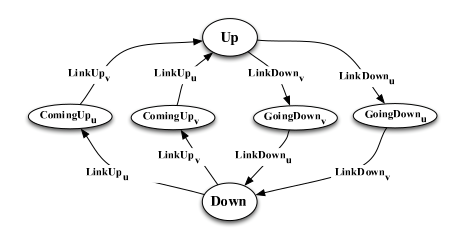
\includegraphics[scale=.75]{screenshot_1.png}
\caption{State diagram for status variable of Link\lbrace u, v\rbrace .}
\end{figure}

If the status is ComingUp u , then messages in transit from u to v are held in the queue until v has been notified that the link is Up. Once the link is Up, the event by which node u receives the message at the head of mqueue v,u is enabled to occur. An attempt by node v to send a message to node u is handled analogously.

Whenever a LinkDown u or LinkDown v event occurs, both message queues are emptied. Neither u nor v is alerted to which messages in transit have been lost due to the LinkDown.

In an initial state of the link, both message queues are empty and the status is either Up or Down.

\section{Configurations and Executions}
The notion of configuration is used to capture an instan-
taneous snapshot of the state of the entire system. A config-
uration is a vector of node states, one for each node in P,
and a vector of link states, one for each link in L .
Assume that the undirected graph G = (V, E) defines the
initial communication topology of the system, where V is a
set of vertices corresponding to the set P of nodes, and E
is a set of edges corresponding to the set of communication
links that are up. In an initial configuration with respect
to G, each node is in an initial state (as prescribed by the
node’s algorithm), each link corresponding to an edge in E
is in an initial state with its status equal to Up, and every
other link has its status equal to Down.
Define an execution as an infinite sequence
C 0 , e 1 ,C 1 , e 2 ,C 2 , . . . of alternating configurations and
events, starting with an initial configuration and, if finite,
ending with a configuration, that satisfies the following
safety conditions:
\begin{itemize}
\item C 0 is an initial configuration (w.r.t. some initial topology G).
\item The preconditions for event are true in $C_{i-1}$ for all $i\geq 1$^.
\item C i is the result of executing event e i on configuration C i−1 , for all i ≥ 1 (only the node and link involved in an event change state, and they change according to their state machine transitions).
\end{itemize}

An execution also satisfies the following liveness condi-
tions:
\begin{itemize}
\item If a link remains Up for infinitely long, then every message sent over the link is eventually delivered.
\item For each link, if only a finite number of link events occur, then the link status after the last one is either Up or Down (not in between).
\end{itemize}

We also assign a positive real-valued global time gt to each event e i , i ≥ 1, such that gt(e i ) < gt(e i+1 ) and, if the execution is infinite, the global times increase without bound. Each configuration inherits the global time of its preceding event, so gt(C i ) = gt(e i ) for i ≥ 1; we define gt(C 0 ) to be 0. We assume that the nodes do not have access to gt.

\section{Problem Definition}
Each node u in the system has a local variable lid u to hold the identifier of the node currently considered by u to be the leader of the connected component containing u.

In every execution that includes a finite number of topology changes, we require that the following eventually holds:
Every connected component CC of the final topology contains a node l, the leader, such that lid u = l for all nodes u ∈ CC, including l itself.

Our algorithm also ensures that eventually each link in the system has a direction imposed on it by virtue of the data stored at each endpoint such that each connected component CC is a leader-oriented DAG, i.e., every node has a directed path to the leader.

\chapter{Sample Title}

Lorem ipsum dolor sit amet, consectetur adipiscing elit, sed do eiusmod tempor incididunt ut labore et dolore magna aliqua. Ut enim ad minim veniam, quis nostrud exercitation ullamco laboris nisi ut aliquip ex ea commodo consequat. Duis aute irure dolor in reprehenderit in voluptate velit esse cillum dolore eu fugiat nulla pariatur. Excepteur sint occaecat cupidatat non proident, sunt in culpa qui officia deserunt mollit anim id est laborum.

%now enable appendix numbering format and include any appendices
\appendix
\chapter{Sample Title}

Lorem ipsum dolor sit amet, consectetur adipiscing elit, sed do eiusmod tempor incididunt ut labore et dolore magna aliqua. Ut enim ad minim veniam, quis nostrud exercitation ullamco laboris nisi ut aliquip ex ea commodo consequat. Duis aute irure dolor in reprehenderit in voluptate velit esse cillum dolore eu fugiat nulla pariatur. Excepteur sint occaecat cupidatat non proident, sunt in culpa qui officia deserunt mollit anim id est laborum.
\chapter{Sample Title}

Lorem ipsum dolor sit amet, consectetur adipiscing elit, sed do eiusmod tempor incididunt ut labore et dolore magna aliqua. Ut enim ad minim veniam, quis nostrud exercitation ullamco laboris nisi ut aliquip ex ea commodo consequat. Duis aute irure dolor in reprehenderit in voluptate velit esse cillum dolore eu fugiat nulla pariatur. Excepteur sint occaecat cupidatat non proident, sunt in culpa qui officia deserunt mollit anim id est laborum.

%next line adds the Bibliography to the contents page
\addcontentsline{toc}{chapter}{Bibliography}
%uncomment next line to change bibliography name to references
%\renewcommand{\bibname}{References}
\bibliography{refs}        %use a bibtex bibliography file refs.bib
\bibliographystyle{plain}  %use the plain bibliography style

\end{document}

